\setlength\intextsep{0pt}
\begin{wrapfigure}{R}{1.0\textwidth}
\begin{minipage}{1.0\textwidth}
\begin{algorithm}[H]
\begin{algorithmic}[1]
     \INPUT primary dataset $\mathcal{P}=\{\bm{x}_i\}^n_{i=1}$, auxiliary dataset $\mathcal{A} = \{\widetilde\bx_j\}_{j=1}^m$, classifier $f(\bm{x}, \bm{w})$, initial weights $\bw_0$, loss function $\mathcal{L}$, learning rate $\eta_t$, option $o\in$\{\texttt{relative}, \texttt{kernelized}\}
     %\State Initialize 
     % $\mathcal{N}=\text{CollectauxiliaryExamples}(\mathcal{P}, N)$
     %auxiliary dataset $\mathcal{N}=\{\bm{x_i}\}^{N}_{i=1}$
     \State combine $\mathcal{D}=\{(\bm{x}_i, y_i=1)$ for $\bm{x}_i \in \mathcal{P}\}\bigcup\{(\bm{x}_i, y_i=-1)$ for $\bm{x}_i \in \mathcal{A}\}$
     %%\State $\bm{w_0}=\text{ParameterInitialize}(f, \mathcal{D}, \mathcal{L})$
     \State set $S$ to $n \times n$ matrix of all zeros
     \For{$t = 1$ to $n+m$}
        %\State $S_{epoch}=[\ ]$
        %\For{$(\bm{x_i}, y_i)\in\mathcat{D}$}
            \State sample $(\bx, y)$ from $\mathcal{D}$ w/o replacement
            \State $\bm{w_t}=\texttt{SGD}(\bm{w}_{t-1}, \bm{x}, y, f, \mathcal{L}, \eta_t)$
            \If{$y=1$}
                \State $\mbf{p}_t=\texttt{Predict}(\mbf{w}_t, \mathcal{P}, f)$
                \State find $1 \le i \le n$ such that $\bx = \bx_i \in \mathcal{P}$
                \If{$o = \texttt{relative}$}
                    \State $\bm{s}_t=\frac{\left| \bm{p}_t-\bm{p}_{t-1} \right|}{\left| \bm{p}_t(i)-\bm{p}_{t-1}(i) \right|}$
                \Else
                    \State $g_t=\texttt{GetGradient}(\bm{w}_{t-1}, \bm{x}, y, f, \mathcal{L})$
                    \State 
                    $\bm{s}_t= \frac{\mbf{p}_t - \mbf{p}_{t-1}}{-\eta_t \times g_t}$
                \EndIf
            \EndIf
            \State set the $i$th row $S(i,:) = \mbf{s}_t$
        %\EndFor
        %\State $S = S + S_{epoch}$
     \EndFor
     %\State $S = \frac{1}{M}S$
     \State $\Sy = \frac{1}{2}(S + S^\top)$
     \State $\bm{y}_{\text{subclass}}=\text{Clustering}(\Sy)$
     %\If{$o$ = retative}
     %   \State $Y_{\text{fine-grained}}=\text{$K$-means}(S_{sym})$
     %\Etse
     %   \State $Y_{\text{fine-grained}}=\text{Kernet $K$-means}(S_{sym})$
     %\EndIf
     \State {\bf return} $\bm{y}_{\text{subclass}}$
\end{algorithmic}
	\caption{The Local Elasticity Based Clustering Algorithm.}
	\label{algo:clustering}
\end{algorithm}
\end{minipage}
\end{wrapfigure}
\section{The Local Elasticity Algorithm for Clustering}
\label{sec:local-elast-based}
%\begin{algorithm}
%\begin{algorithmic}
% 	\DontPrintSemicolon % Some LaTeX compilers require you to use \dontprintsemicolon instead
%	\State {\bf Input:} unlabeled data $\mathcal{U}$=$\{\mbf{x}_i\}_{i=1}^N$, initialized parameters of neural nets $\mbf{w}_0$, loss function $l$, learning rate $\eta$, method option $mo$
%	\State Initialize $M=\{\}$
%	\For{$i = 1$ to $N$}
%	    \State $\mbf{p}_0$ = Inference($\mbf{w}_0$, $\mathcal{U}$)
%	    \State $\mbf{w}_i$ = SGDUpdate($\mbf{w}_0$, $\mbf{x}_i$, $y_i =1$)
%	    \State $\mbf{p}_i$ = Inference($\mbf{w}_i$, $\mathcal{U}$)
%	\If{$mo = kernel$}
%	    \State $c_i$ = LossGradient($l$, $\mbf{w}_0$, $\mbf{x}_i$, $y_i=1$)
%	    \State $\mbf{v}_i = \frac{\mbf{p}_i - \mbf{p}_0}{-\eta \times c_i}$
%	\Else
%	    \State $\mbf{v}_i = \frac{\mbf{p}_i - \mbf{p}_0}{\mbf{p}_i[i] - \mbf{p}_0[i]}$
%	\EndIf
%	\State $M$ = Extend($M$, $\mbf{v}_i$) 
%	\EndFor
%	\State $\hat{Y}$ = $K$-means($M$) \weijie{be careful. one is normal kmeans, the other is kernel kmeans.}
%\end{algorithmic}
%	\caption{Local Elasticity Based Clustering Algorithm. \weijie{The description needs to mention it can incorporate multiple epochs, and use $L$ to denote the loss, and mention the symmetrization. }}
%	\label{algo:clustering}
%\end{algorithm}
This section introduces a novel algorithm for clustering that leverages the local elasticity of neural networks. We focus on the setting where all (primary) examples are from the same (known) superclass (e.g., mammal) and the interest is, however, to partition the primary examples into finer-grained (unknown) classes (e.g., cat and dog). To facilitate this process, we include an auxiliary dataset with all examples from a different superclass (e.g., vehicle). See Figure~\ref{fig:clustering} for an illustration of the setting. To clear off any confusion, we remark that the aim is to corroborate the hypothesis of local elasticity by showing the effectiveness of this clustering algorithm. 

%%For instance, considering a dataset whose samples are each labeled as mammal or vehicle, and the goal is to cluster the mammal part into cat or dog while to cluster the vehicle part into car or truck as shown in Figure \ref{fig:clustering}.

%\begin{figure}[!htp]%%{r}{0.25\textwidth}
%  \begin{center}
%	  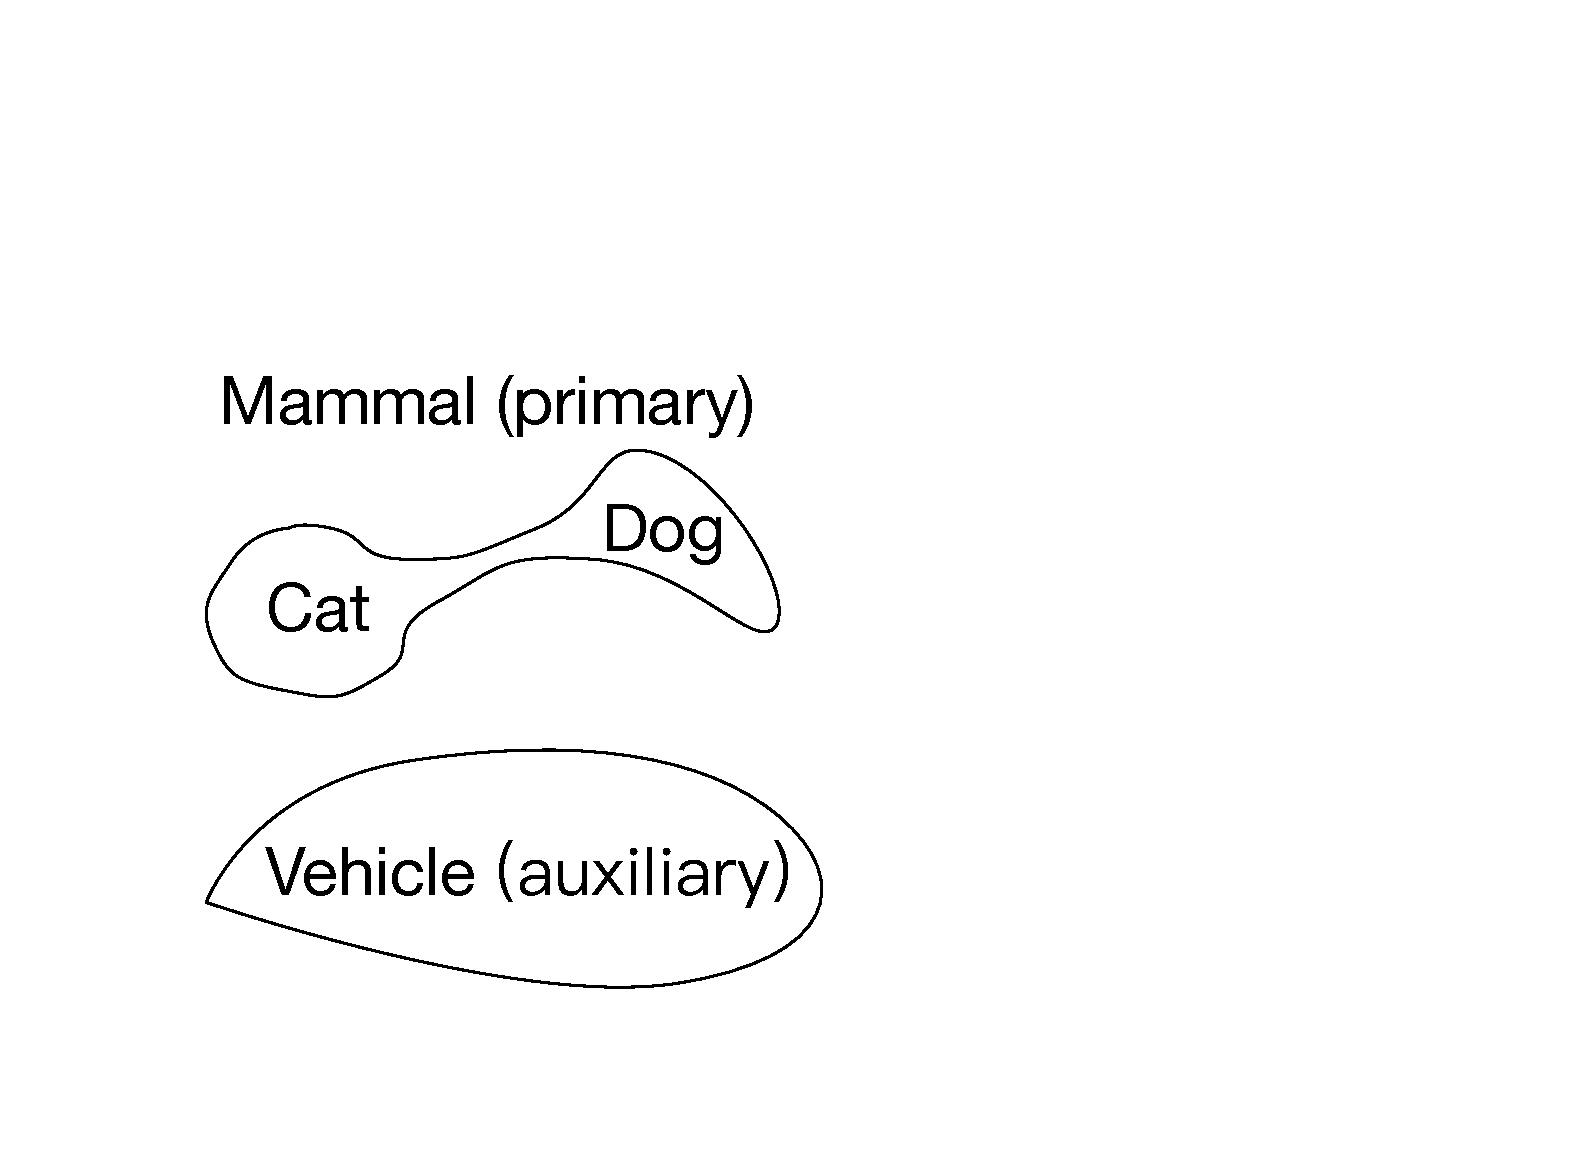
\includegraphics[scale=0.3]{Figures/clusters.pdf}
%  \end{center}
%  \caption{Illustration of the primary dataset and auxiliary dataset taken as input of the local elasticity based clustering algorithm. 
 % %When grouping samples into super classes, mammal and vehicle, neural nets can automatically cluster samples into subgroups within one super class, based on the local elasticity. Figures are shown for illustration purposes only.
%  }
%  \label{fig:clustering}
%\end{figure}
The centerpiece of our algorithm is the dynamic construction of a matrix that records pairwise similarities between all primary examples. In brief, the algorithm operates as if it were learning to distinguish between the primary examples (e.g., mammals) and the auxiliary examples (e.g., vehicles) via SGD. On top of that, the algorithm evaluates the changes in the predictions for any pairs of primary examples during the training process, and the recorded changes are used to construct the pairwise similarity matrix based on either the relative similarity in Equation (\ref{eq:sr}) or the kernelized similarity in Equation (\ref{eq:sk}). Taking the mammal case as earlier, the rationale of the algorithm is that local elasticity is likely to yield a larger similarity score between two cats (or two dogs), and a smaller similarity score between a cat and a dog.

%%Within the mammal class, two images of cats are more likely to have a larger similarity score than those of a cat and a dog, and this fact is expected to be captured by the local elasticity of the networks. The algorithm learns the super class as usual while, in an unsupervised way, clusters the samples into subgroups. This appealing feature of this proposal allows for easy implementation in most deep learning platforms. This method is presented in Algorithm \ref{algo:clustering}, with some elaboration for more details below.

%%\setlength\intextsep{0pt}
\begin{wrapfigure}{r}{0.28\textwidth}
  \begin{center}
	  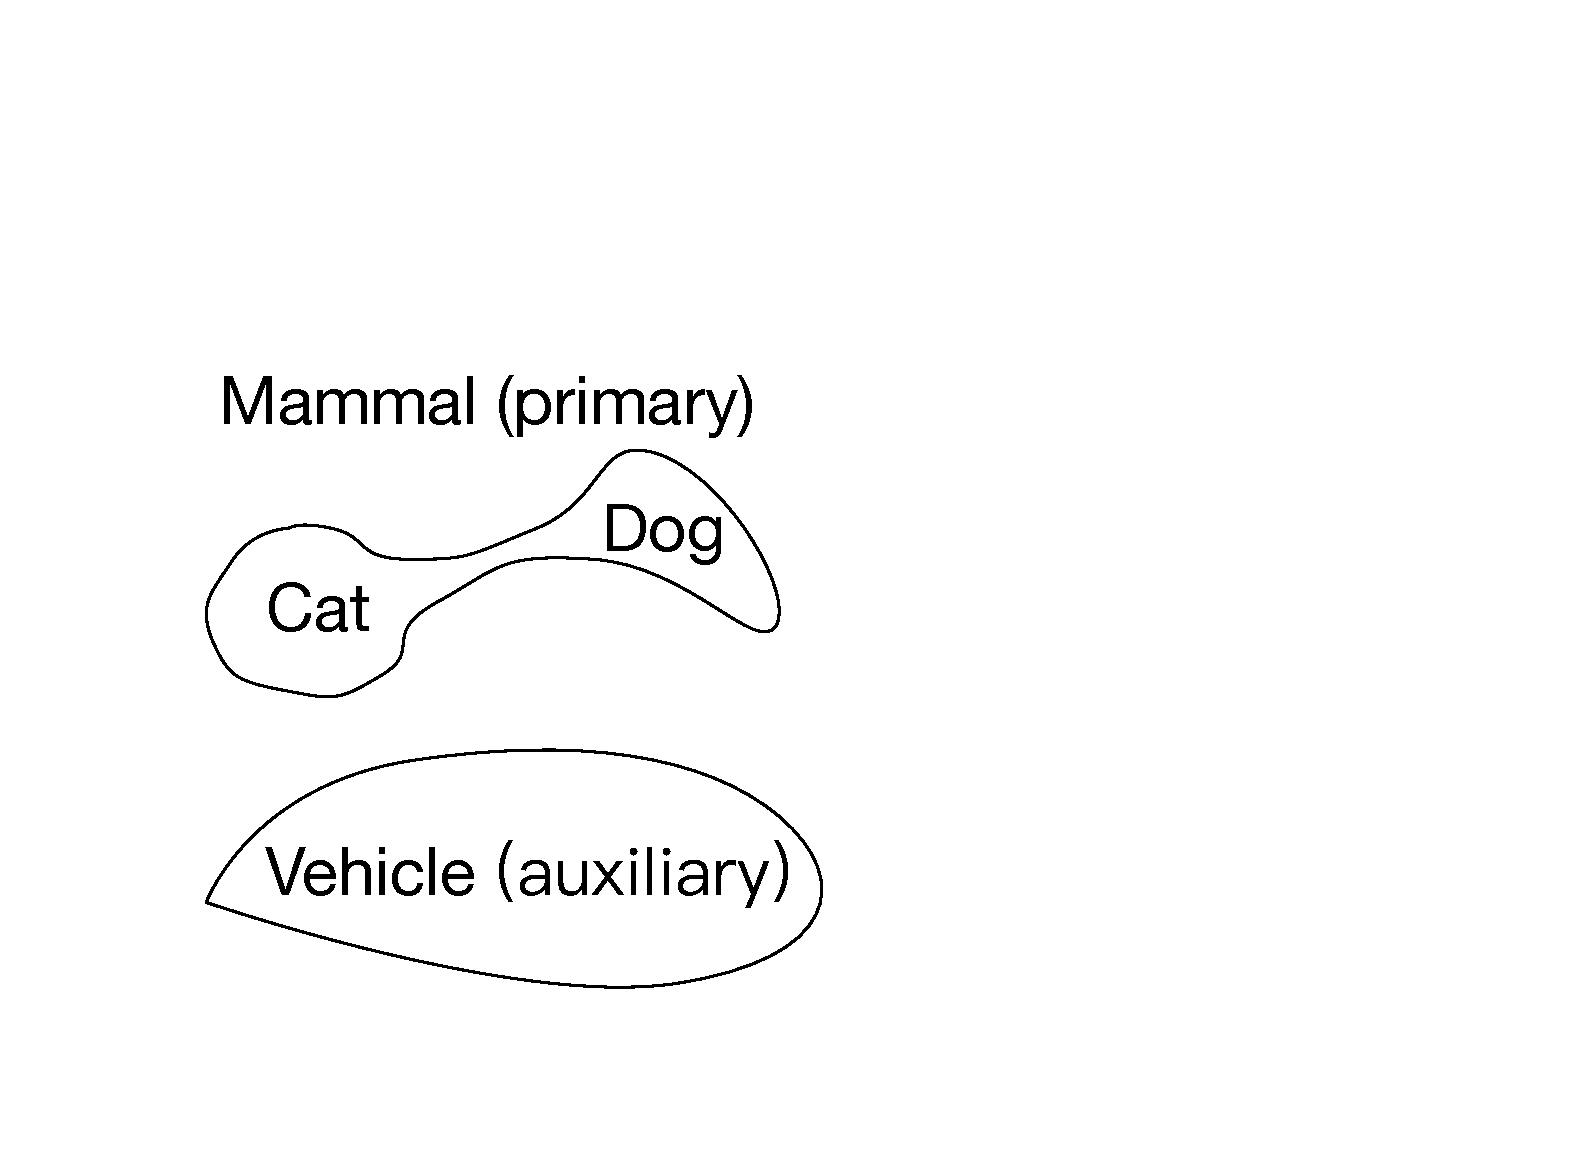
\includegraphics[scale=0.35]{Figures/clusters.pdf}
  \end{center}
  \caption{Illustration of the primary dataset and auxiliary dataset taken as input by the local elasticity based clustering algorithm. 
  %When grouping samples into super classes, mammal and vehicle, neural nets can automatically cluster samples into subgroups within one super class, based on the local elasticity. Figures are shown for illustration purposes only.
  }
  \label{fig:clustering}
\end{wrapfigure}
This method is formally presented in Algorithm \ref{algo:clustering}, with elaboration as follows. While the initial parameters $\bw_0$ are often set to i.i.d.~random variables, our experiments suggest that ``pre-trained'' weights can lead to better clustering performance. Hence, we use a warm-up period to get nearly optimal $\bw_0$ by training on the combined dataset $\mathcal{D}$. When the SGD is performed at a primary example $\bx_i$ (labeled $y_i = 1$) during the iterations, the function \texttt{Predict}$(\bw_i, \mathcal{P}, f) \in \R^n$ evaluates the predictions for all primary examples at $\bw_i$, and these results are used to compute similarity measures between $\bx_i$ and other primary feature vectors using Equation (\ref{eq:sr}) or Equation (\ref{eq:sk}), depending on the option. If one chooses to use the kernelized similarity, the function $\texttt{GetGradient}$ is called to the gradient of the loss function $\mathcal{L}$ at $\bw_{t-1}, (\bx, y)$ with respect to $f$. In practice, we can repeat the loop multiple times and then average the similarity matrices over the epochs. Finally, using the symmetrized $\Sy$, we apply an off-the-shelf clustering method such as $K$-means (for relative similarity) or kernel $K$-means (for kernel similarity) to partition the primary dataset $\mathcal{P}$ into subclasses.

% After that, we average the similarity matrices among $M$ epochs to get the average similarity matrix $S$ in line $22$. The final symmetric similarity matrix $S_{sym}$ is obtained by averaging $S$ and its transpose $S^T$ in line $23$. Finally, primary examples in $\mathcal{P}$ are clustered into fine-grained classes based on relative similarity or kernelized similarity between each other (line $24$). 
% Predict($\mbf{w}$, $\mathcal{D}$, $f$) is used to get the predictions of the net $f(\mbf{x}, \mbf{w})$ on the whole data $\mathcal{D}$ with the parameters $\mbf{w}$, so the output is a vector of predictions.
% In our experiments, we use $K$-means for relative similarity based clustering algorithms, and kernel $K$-means for kernelized similarity based clustering algorithms. Our algorithm can be further improved by using a more customized clustering method for the similarity matrix. 
% %%either the kernelized similarity vector between the updated point $x$ and the primary examples $\mathcal{P}$ is computed in line $11$-$16$. In this way, 
%%we can get a similarity matrix $S_{epoch}$ for each epoch. 

%%The clustering algorithm based on the local elasticity relies on the choice of parameters $\mbf{w}$. We consider using the examples of other classes to get a nearly optimal estimation.Specifically, we use ParameterInitialize($f$, $\mathcal{D}$, $\mathcal{L}$) to initialize the parameters $\mbf{w}$ of the net $f(\mbf{x}, \mbf{w})$ according to the dataset $\mathcal{D}$ and the loss function $\mathcal{L}$.


%%If the SGD is performed at a primary example, which is labeled $y_i = 1$, For each SGD update on $\mathcal{P}$, a relative or kernelized similarity vector between the updated point $x$ and the primary examples $\mathcal{P}$ is computed in line $11$-$16$. In this way, we can get a similarity matrix $S_{epoch}$ for each epoch. After that, we average the similarity matrices among $M$ epochs to get the average similarity matrix $S$ in line $22$. The final symmetric similarity matrix $S_{sym}$ is obtained by averaging $S$ and its transpose $S^T$ in line $23$. Finally, primary examples in $\mathcal{P}$ are clustered into fine-grained classes based on relative similarity or kernelized similarity between each other (line $24$). 




%Throughout the procedure, we use five oracles: ParameterInitialize, BackPropagate, Predict, GetLossGradient and Clustering. 

%{\bf BackPropagation.} BackPropagate function updates the parameters $\mbf{w}$ of the net $f(\mbf{x}, \mbf{w})$ according to the loss function $\mathcal{L}$ and learning rate $\eta$ after a SGD update on the point $(\mbf{x}, y)$. {\bf Loss Gradient.} GetLossGradient($\mbf{w}$, $\mbf{x}$, $y$, $f$, $\mathcal{L}$) computes the gradient of loss over the net $f(\mbf{x}, \mbf{w})$ with the parameters $\mbf{w}$ on the point $(\mbf{x}, y)$ according to the loss function $\mathcal{L}$. We only compute the symmetric similarity matrix for primary examples, so the label in Backpropagate and GetLossGradient is always $y=1$.
%%Given primary examples $\mathcal{P}$ from a super class (e.g mammal), we first collect some auxilary examples $\mathcal{N}$ from other super classes (e.g vehicle) to construct a new dataset $\mathcal{D}$ with positive labels for $\mathcal{P}$ and negative labels for $\mathcal{N}$ in line $1$-$2$. We then train the net $f(\mbf{x},\mbf{w})$ on $\mathcal{D}$ to approximate the global minimum of training loss $\mathcal{L}$, and use the parameters $\mbf{w}_0$ as an initial start in line $3$. 
%%{\bf Datasets.} To get the fine-grained classes for the primary examples in the dataset $\mathcal{P}$, we collect $N$ auxiliary examples $\mathcal{N}$ from the super classes that are different from that of the examples in $\mathcal{P}$.

%{\bf Parameter initialization.}
%The clustering algorithm based on the local elasticity relies on the choice of parameters $\mbf{w}$. We consider using the examples of other classes to get a nearly optimal estimation.
%Although NTK is based on random initialized parameters, we also consider using the examples of other classes to get a nearly optimal estimation. For example, assume we want to cluster the data into two types, dog and cat. We first treat samples in both the dog and cat classes as primary examples (mammal), and then consider samples in car and truck classes as auxiliary examples (vehicle) to learn a nearly optimal estimation for parameters. This is based on the intuition that we can learn detailed features of primary examples to better distinguish them from auxiliary examples. Further analysis can be found in Section \ref{subsec:results}. 
%%Specifically, we use ParameterInitialize($f$, $\mathcal{D}$, $\mathcal{L}$) to initialize the parameters $\mbf{w}$ of the net $f(\mbf{x}, \mbf{w})$ according to the dataset $\mathcal{D}$ and the loss function $\mathcal{L}$.

%{\bf Prediction.}
%Predict($\mbf{w}$, $\mathcal{D}$, $f$) is used to get the predictions of the net $f(\mbf{x}, \mbf{w})$ on the whole data $\mathcal{D}$ with the parameters $\mbf{w}$, so the output is a vector of predictions.

%{\bf Clustering algorithm.}
%%In our experiments, we use $K$-means for relative similarity based clustering algorithms, and kernel $K$-means for kernelized similarity based clustering algorithms. Our algorithm can be further improved by using a more customized clustering method for the similarity matrix. 

%%Although we simply consider two clusters here, it is easy to expand the number of clusters.


%%% Local Variables:
%%% mode: latex
%%% TeX-master: "paper"
%%% End:
